\documentclass[twoside]{book}

% Packages required by doxygen
\usepackage{fixltx2e}
\usepackage{calc}
\usepackage{doxygen}
\usepackage[export]{adjustbox} % also loads graphicx
\usepackage{graphicx}
\usepackage[utf8]{inputenc}
\usepackage{makeidx}
\usepackage{multicol}
\usepackage{multirow}
\PassOptionsToPackage{warn}{textcomp}
\usepackage{textcomp}
\usepackage[nointegrals]{wasysym}
\usepackage[table]{xcolor}

% Font selection
\usepackage[T1]{fontenc}
\usepackage[scaled=.90]{helvet}
\usepackage{courier}
\usepackage{amssymb}
\usepackage{sectsty}
\renewcommand{\familydefault}{\sfdefault}
\allsectionsfont{%
  \fontseries{bc}\selectfont%
  \color{darkgray}%
}
\renewcommand{\DoxyLabelFont}{%
  \fontseries{bc}\selectfont%
  \color{darkgray}%
}
\newcommand{\+}{\discretionary{\mbox{\scriptsize$\hookleftarrow$}}{}{}}

% Page & text layout
\usepackage{geometry}
\geometry{%
  a4paper,%
  top=2.5cm,%
  bottom=2.5cm,%
  left=2.5cm,%
  right=2.5cm%
}
\tolerance=750
\hfuzz=15pt
\hbadness=750
\setlength{\emergencystretch}{15pt}
\setlength{\parindent}{0cm}
\setlength{\parskip}{3ex plus 2ex minus 2ex}
\makeatletter
\renewcommand{\paragraph}{%
  \@startsection{paragraph}{4}{0ex}{-1.0ex}{1.0ex}{%
    \normalfont\normalsize\bfseries\SS@parafont%
  }%
}
\renewcommand{\subparagraph}{%
  \@startsection{subparagraph}{5}{0ex}{-1.0ex}{1.0ex}{%
    \normalfont\normalsize\bfseries\SS@subparafont%
  }%
}
\makeatother

% Headers & footers
\usepackage{fancyhdr}
\pagestyle{fancyplain}
\fancyhead[LE]{\fancyplain{}{\bfseries\thepage}}
\fancyhead[CE]{\fancyplain{}{}}
\fancyhead[RE]{\fancyplain{}{\bfseries\leftmark}}
\fancyhead[LO]{\fancyplain{}{\bfseries\rightmark}}
\fancyhead[CO]{\fancyplain{}{}}
\fancyhead[RO]{\fancyplain{}{\bfseries\thepage}}
\fancyfoot[LE]{\fancyplain{}{}}
\fancyfoot[CE]{\fancyplain{}{}}
\fancyfoot[RE]{\fancyplain{}{\bfseries\scriptsize Generated by Doxygen }}
\fancyfoot[LO]{\fancyplain{}{\bfseries\scriptsize Generated by Doxygen }}
\fancyfoot[CO]{\fancyplain{}{}}
\fancyfoot[RO]{\fancyplain{}{}}
\renewcommand{\footrulewidth}{0.4pt}
\renewcommand{\chaptermark}[1]{%
  \markboth{#1}{}%
}
\renewcommand{\sectionmark}[1]{%
  \markright{\thesection\ #1}%
}

% Indices & bibliography
\usepackage{natbib}
\usepackage[titles]{tocloft}
\setcounter{tocdepth}{3}
\setcounter{secnumdepth}{5}
\makeindex

% Hyperlinks (required, but should be loaded last)
\usepackage{ifpdf}
\ifpdf
  \usepackage[pdftex,pagebackref=true]{hyperref}
\else
  \usepackage[ps2pdf,pagebackref=true]{hyperref}
\fi
\hypersetup{%
  colorlinks=true,%
  linkcolor=blue,%
  citecolor=blue,%
  unicode%
}

% Custom commands
\newcommand{\clearemptydoublepage}{%
  \newpage{\pagestyle{empty}\cleardoublepage}%
}

\usepackage{caption}
\captionsetup{labelsep=space,justification=centering,font={bf},singlelinecheck=off,skip=4pt,position=top}

%===== C O N T E N T S =====

\begin{document}

% Titlepage & ToC
\hypersetup{pageanchor=false,
             bookmarksnumbered=true,
             pdfencoding=unicode
            }
\pagenumbering{alph}
\begin{titlepage}
\vspace*{7cm}
\begin{center}%
{\Large Project 6 }\\
\vspace*{1cm}
{\large Generated by Doxygen 1.8.14}\\
\end{center}
\end{titlepage}
\clearemptydoublepage
\pagenumbering{roman}
\tableofcontents
\clearemptydoublepage
\pagenumbering{arabic}
\hypersetup{pageanchor=true}

%--- Begin generated contents ---
\chapter{Hierarchical Index}
\section{Class Hierarchy}
This inheritance list is sorted roughly, but not completely, alphabetically\+:\begin{DoxyCompactList}
\item \contentsline{section}{Node}{\pageref{class_node}}{}
\begin{DoxyCompactList}
\item \contentsline{section}{Node\+Tree}{\pageref{class_node_tree}}{}
\end{DoxyCompactList}
\end{DoxyCompactList}

\chapter{Class Index}
\section{Class List}
Here are the classes, structs, unions and interfaces with brief descriptions\+:\begin{DoxyCompactList}
\item\contentsline{section}{\mbox{\hyperlink{classarray_list}{array\+List}} }{\pageref{classarray_list}}{}
\item\contentsline{section}{\mbox{\hyperlink{classlinked_list}{linked\+List}} }{\pageref{classlinked_list}}{}
\item\contentsline{section}{\mbox{\hyperlink{classqueue}{queue}} }{\pageref{classqueue}}{}
\item\contentsline{section}{\mbox{\hyperlink{classqueue_linked}{queue\+Linked}} }{\pageref{classqueue_linked}}{}
\end{DoxyCompactList}

\chapter{Class Documentation}
\hypertarget{class_node}{}\section{Node Class Reference}
\label{class_node}\index{Node@{Node}}
Inheritance diagram for Node\+:\begin{figure}[H]
\begin{center}
\leavevmode
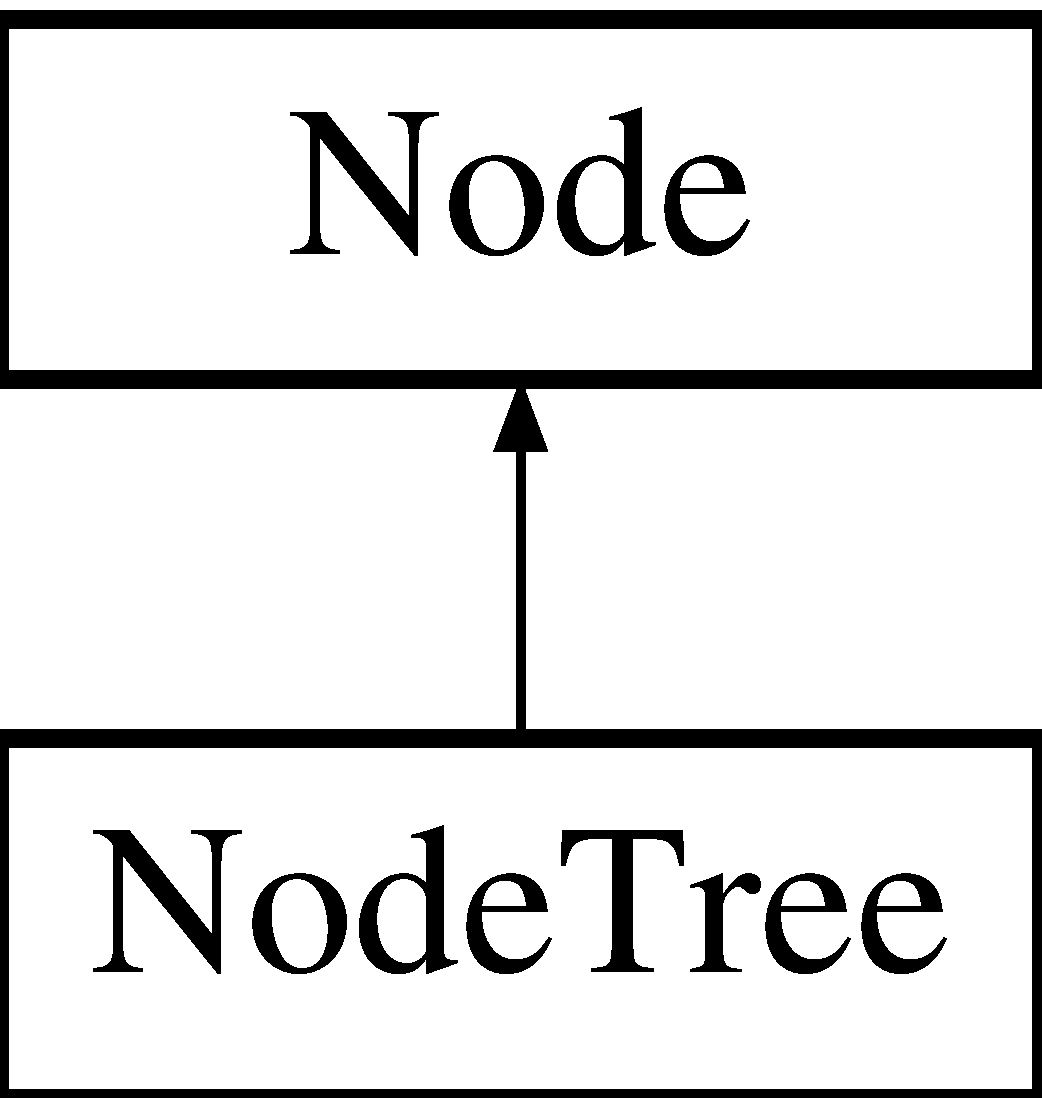
\includegraphics[height=2.000000cm]{class_node}
\end{center}
\end{figure}
\subsection*{Public Member Functions}
\begin{DoxyCompactItemize}
\item 
\mbox{\Hypertarget{class_node_ad7a34779cad45d997bfd6d3d8043c75f}\label{class_node_ad7a34779cad45d997bfd6d3d8043c75f}} 
\mbox{\hyperlink{class_node_ad7a34779cad45d997bfd6d3d8043c75f}{Node}} ()
\begin{DoxyCompactList}\small\item\em Default Constructor for \mbox{\hyperlink{class_node}{Node}}. \end{DoxyCompactList}\item 
\mbox{\hyperlink{class_node_a6b85d29b3bde0f983d0a6135ca440c0a}{Node}} (const int \&anitem)
\item 
\mbox{\hyperlink{class_node_a63f4f5083e2a677525a28a5cd194178d}{Node}} (const int \&item, \mbox{\hyperlink{class_node}{Node}} $\ast$left\+Ptr, \mbox{\hyperlink{class_node}{Node}} $\ast$right\+Ptr)
\begin{DoxyCompactList}\small\item\em Constructor for item, and the child objects. \end{DoxyCompactList}\item 
\mbox{\hyperlink{class_node}{Node}} $\ast$ \mbox{\hyperlink{class_node_a2ee7aacc0b20abf2301256fe72d0d9cc}{set\+Item}} (const int \&anitem)
\begin{DoxyCompactList}\small\item\em Will set the value for the item. \end{DoxyCompactList}\item 
int \mbox{\hyperlink{class_node_ad51c74ff8860a12738136be8f1f17682}{get\+Item}} ()
\begin{DoxyCompactList}\small\item\em Will return the item value at that node. \end{DoxyCompactList}\item 
\mbox{\Hypertarget{class_node_aa4852cb11b6fc5fbb03e110390d0966d}\label{class_node_aa4852cb11b6fc5fbb03e110390d0966d}} 
void {\bfseries set\+Count} ()
\item 
\mbox{\Hypertarget{class_node_a7fa9c0a066de25a23670691f6ca99116}\label{class_node_a7fa9c0a066de25a23670691f6ca99116}} 
int {\bfseries get\+Count} ()
\item 
bool \mbox{\hyperlink{class_node_a0c5b662d3bfbb856292a9aab878ed622}{is\+Leaf}} () const
\begin{DoxyCompactList}\small\item\em Whill cheak if that node has leaft values. \end{DoxyCompactList}\item 
\mbox{\hyperlink{class_node}{Node}} $\ast$ \mbox{\hyperlink{class_node_a81c225637a0cc1edd73c2aba18ea6f4a}{get\+Left\+Child\+Ptr}} ()
\begin{DoxyCompactList}\small\item\em Will return the left child pointer at that node. \end{DoxyCompactList}\item 
\mbox{\hyperlink{class_node}{Node}} $\ast$ \mbox{\hyperlink{class_node_a9f9db183586c193a33627e239b1cdab5}{get\+Right\+Child\+Ptr}} ()
\begin{DoxyCompactList}\small\item\em Will return the right child pointer at that node. \end{DoxyCompactList}\item 
void \mbox{\hyperlink{class_node_a4da6acb58d5b8f60bc7ac822250cda32}{set\+Left\+Child\+Ptr}} (\mbox{\hyperlink{class_node}{Node}} $\ast$left\+Ptr)
\begin{DoxyCompactList}\small\item\em Will set the left child pointer for the item. \end{DoxyCompactList}\item 
void \mbox{\hyperlink{class_node_a7e4994f0037bcc6b52a568de0c0a8acf}{set\+Right\+Child\+Ptr}} (\mbox{\hyperlink{class_node}{Node}} $\ast$right\+Ptr)
\begin{DoxyCompactList}\small\item\em Will set the right child pointer for the node. \end{DoxyCompactList}\end{DoxyCompactItemize}


\subsection{Constructor \& Destructor Documentation}
\mbox{\Hypertarget{class_node_a6b85d29b3bde0f983d0a6135ca440c0a}\label{class_node_a6b85d29b3bde0f983d0a6135ca440c0a}} 
\index{Node@{Node}!Node@{Node}}
\index{Node@{Node}!Node@{Node}}
\subsubsection{\texorpdfstring{Node()}{Node()}\hspace{0.1cm}{\footnotesize\ttfamily [1/2]}}
{\footnotesize\ttfamily Node\+::\+Node (\begin{DoxyParamCaption}\item[{const int \&}]{anitem }\end{DoxyParamCaption})}

Constructor for the item only 
\begin{DoxyParams}{Parameters}
{\em anitem} & \\
\hline
\end{DoxyParams}
\begin{DoxyPrecond}{Precondition}
Will take in an int to give to the item 
\end{DoxyPrecond}
\begin{DoxyPostcond}{Postcondition}
Will give the set the item to the value and set the childs to null 
\end{DoxyPostcond}
\mbox{\Hypertarget{class_node_a63f4f5083e2a677525a28a5cd194178d}\label{class_node_a63f4f5083e2a677525a28a5cd194178d}} 
\index{Node@{Node}!Node@{Node}}
\index{Node@{Node}!Node@{Node}}
\subsubsection{\texorpdfstring{Node()}{Node()}\hspace{0.1cm}{\footnotesize\ttfamily [2/2]}}
{\footnotesize\ttfamily Node\+::\+Node (\begin{DoxyParamCaption}\item[{const int \&}]{anitem,  }\item[{\mbox{\hyperlink{class_node}{Node}} $\ast$}]{left\+Ptr,  }\item[{\mbox{\hyperlink{class_node}{Node}} $\ast$}]{right\+Ptr }\end{DoxyParamCaption})}



Constructor for item, and the child objects. 


\begin{DoxyParams}{Parameters}
{\em anitem} & \\
\hline
{\em left\+Ptr} & \\
\hline
{\em right\+Ptr} & \\
\hline
\end{DoxyParams}
\begin{DoxyPrecond}{Precondition}
Will take the item and child pointer values 
\end{DoxyPrecond}


\subsection{Member Function Documentation}
\mbox{\Hypertarget{class_node_ad51c74ff8860a12738136be8f1f17682}\label{class_node_ad51c74ff8860a12738136be8f1f17682}} 
\index{Node@{Node}!get\+Item@{get\+Item}}
\index{get\+Item@{get\+Item}!Node@{Node}}
\subsubsection{\texorpdfstring{get\+Item()}{getItem()}}
{\footnotesize\ttfamily int Node\+::get\+Item (\begin{DoxyParamCaption}{ }\end{DoxyParamCaption})}



Will return the item value at that node. 

\begin{DoxyReturn}{Returns}
item 
\end{DoxyReturn}
\begin{DoxyPrecond}{Precondition}
Will get called at that node 
\end{DoxyPrecond}
\begin{DoxyPostcond}{Postcondition}
Will return the value at that node 
\end{DoxyPostcond}
\mbox{\Hypertarget{class_node_a81c225637a0cc1edd73c2aba18ea6f4a}\label{class_node_a81c225637a0cc1edd73c2aba18ea6f4a}} 
\index{Node@{Node}!get\+Left\+Child\+Ptr@{get\+Left\+Child\+Ptr}}
\index{get\+Left\+Child\+Ptr@{get\+Left\+Child\+Ptr}!Node@{Node}}
\subsubsection{\texorpdfstring{get\+Left\+Child\+Ptr()}{getLeftChildPtr()}}
{\footnotesize\ttfamily \mbox{\hyperlink{class_node}{Node}} $\ast$ Node\+::get\+Left\+Child\+Ptr (\begin{DoxyParamCaption}{ }\end{DoxyParamCaption})}



Will return the left child pointer at that node. 

\begin{DoxyReturn}{Returns}
left\+Child\+Ptr 
\end{DoxyReturn}
\begin{DoxyPrecond}{Precondition}
Will get called at that node 
\end{DoxyPrecond}
\begin{DoxyPostcond}{Postcondition}
Will return the left child pointer at that node 
\end{DoxyPostcond}
\mbox{\Hypertarget{class_node_a9f9db183586c193a33627e239b1cdab5}\label{class_node_a9f9db183586c193a33627e239b1cdab5}} 
\index{Node@{Node}!get\+Right\+Child\+Ptr@{get\+Right\+Child\+Ptr}}
\index{get\+Right\+Child\+Ptr@{get\+Right\+Child\+Ptr}!Node@{Node}}
\subsubsection{\texorpdfstring{get\+Right\+Child\+Ptr()}{getRightChildPtr()}}
{\footnotesize\ttfamily \mbox{\hyperlink{class_node}{Node}} $\ast$ Node\+::get\+Right\+Child\+Ptr (\begin{DoxyParamCaption}{ }\end{DoxyParamCaption})}



Will return the right child pointer at that node. 

\begin{DoxyReturn}{Returns}
right\+Child\+Ptr 
\end{DoxyReturn}
\begin{DoxyPrecond}{Precondition}
Will get called at that node 
\end{DoxyPrecond}
\begin{DoxyPostcond}{Postcondition}
Will return the right child pointer at that node 
\end{DoxyPostcond}
\mbox{\Hypertarget{class_node_a0c5b662d3bfbb856292a9aab878ed622}\label{class_node_a0c5b662d3bfbb856292a9aab878ed622}} 
\index{Node@{Node}!is\+Leaf@{is\+Leaf}}
\index{is\+Leaf@{is\+Leaf}!Node@{Node}}
\subsubsection{\texorpdfstring{is\+Leaf()}{isLeaf()}}
{\footnotesize\ttfamily bool Node\+::is\+Leaf (\begin{DoxyParamCaption}{ }\end{DoxyParamCaption}) const}



Whill cheak if that node has leaft values. 

\begin{DoxyReturn}{Returns}
bool 
\end{DoxyReturn}
\begin{DoxyPrecond}{Precondition}
Will check it that node has leafs 
\end{DoxyPrecond}
\begin{DoxyPostcond}{Postcondition}
Will return a bool value to check the leafs 
\end{DoxyPostcond}
\mbox{\Hypertarget{class_node_a2ee7aacc0b20abf2301256fe72d0d9cc}\label{class_node_a2ee7aacc0b20abf2301256fe72d0d9cc}} 
\index{Node@{Node}!set\+Item@{set\+Item}}
\index{set\+Item@{set\+Item}!Node@{Node}}
\subsubsection{\texorpdfstring{set\+Item()}{setItem()}}
{\footnotesize\ttfamily \mbox{\hyperlink{class_node}{Node}} $\ast$ Node\+::set\+Item (\begin{DoxyParamCaption}\item[{const int \&}]{anitem }\end{DoxyParamCaption})}



Will set the value for the item. 


\begin{DoxyParams}{Parameters}
{\em anitem} & \\
\hline
\end{DoxyParams}
\begin{DoxyPrecond}{Precondition}
Will take in the item value to set it 
\end{DoxyPrecond}
\begin{DoxyPostcond}{Postcondition}
Will set the item to the node item 
\end{DoxyPostcond}
\mbox{\Hypertarget{class_node_a4da6acb58d5b8f60bc7ac822250cda32}\label{class_node_a4da6acb58d5b8f60bc7ac822250cda32}} 
\index{Node@{Node}!set\+Left\+Child\+Ptr@{set\+Left\+Child\+Ptr}}
\index{set\+Left\+Child\+Ptr@{set\+Left\+Child\+Ptr}!Node@{Node}}
\subsubsection{\texorpdfstring{set\+Left\+Child\+Ptr()}{setLeftChildPtr()}}
{\footnotesize\ttfamily void Node\+::set\+Left\+Child\+Ptr (\begin{DoxyParamCaption}\item[{\mbox{\hyperlink{class_node}{Node}} $\ast$}]{left\+Ptr }\end{DoxyParamCaption})}



Will set the left child pointer for the item. 


\begin{DoxyParams}{Parameters}
{\em left\+Ptr} & \\
\hline
\end{DoxyParams}
\begin{DoxyPrecond}{Precondition}
Will take in the pointer value to set it 
\end{DoxyPrecond}
\begin{DoxyPostcond}{Postcondition}
Will set the left child pointer to the node item 
\end{DoxyPostcond}
\mbox{\Hypertarget{class_node_a7e4994f0037bcc6b52a568de0c0a8acf}\label{class_node_a7e4994f0037bcc6b52a568de0c0a8acf}} 
\index{Node@{Node}!set\+Right\+Child\+Ptr@{set\+Right\+Child\+Ptr}}
\index{set\+Right\+Child\+Ptr@{set\+Right\+Child\+Ptr}!Node@{Node}}
\subsubsection{\texorpdfstring{set\+Right\+Child\+Ptr()}{setRightChildPtr()}}
{\footnotesize\ttfamily void Node\+::set\+Right\+Child\+Ptr (\begin{DoxyParamCaption}\item[{\mbox{\hyperlink{class_node}{Node}} $\ast$}]{right\+Ptr }\end{DoxyParamCaption})}



Will set the right child pointer for the node. 


\begin{DoxyParams}{Parameters}
{\em right\+Ptr} & \\
\hline
\end{DoxyParams}
\begin{DoxyPrecond}{Precondition}
Will take in the pointer value to set it 
\end{DoxyPrecond}
\begin{DoxyPostcond}{Postcondition}
Will set the right child pointer to the node 
\end{DoxyPostcond}


The documentation for this class was generated from the following files\+:\begin{DoxyCompactItemize}
\item 
Node.\+h\item 
Node.\+cpp\end{DoxyCompactItemize}

\hypertarget{class_node_tree}{}\section{Node\+Tree Class Reference}
\label{class_node_tree}\index{Node\+Tree@{Node\+Tree}}
Inheritance diagram for Node\+Tree\+:\begin{figure}[H]
\begin{center}
\leavevmode
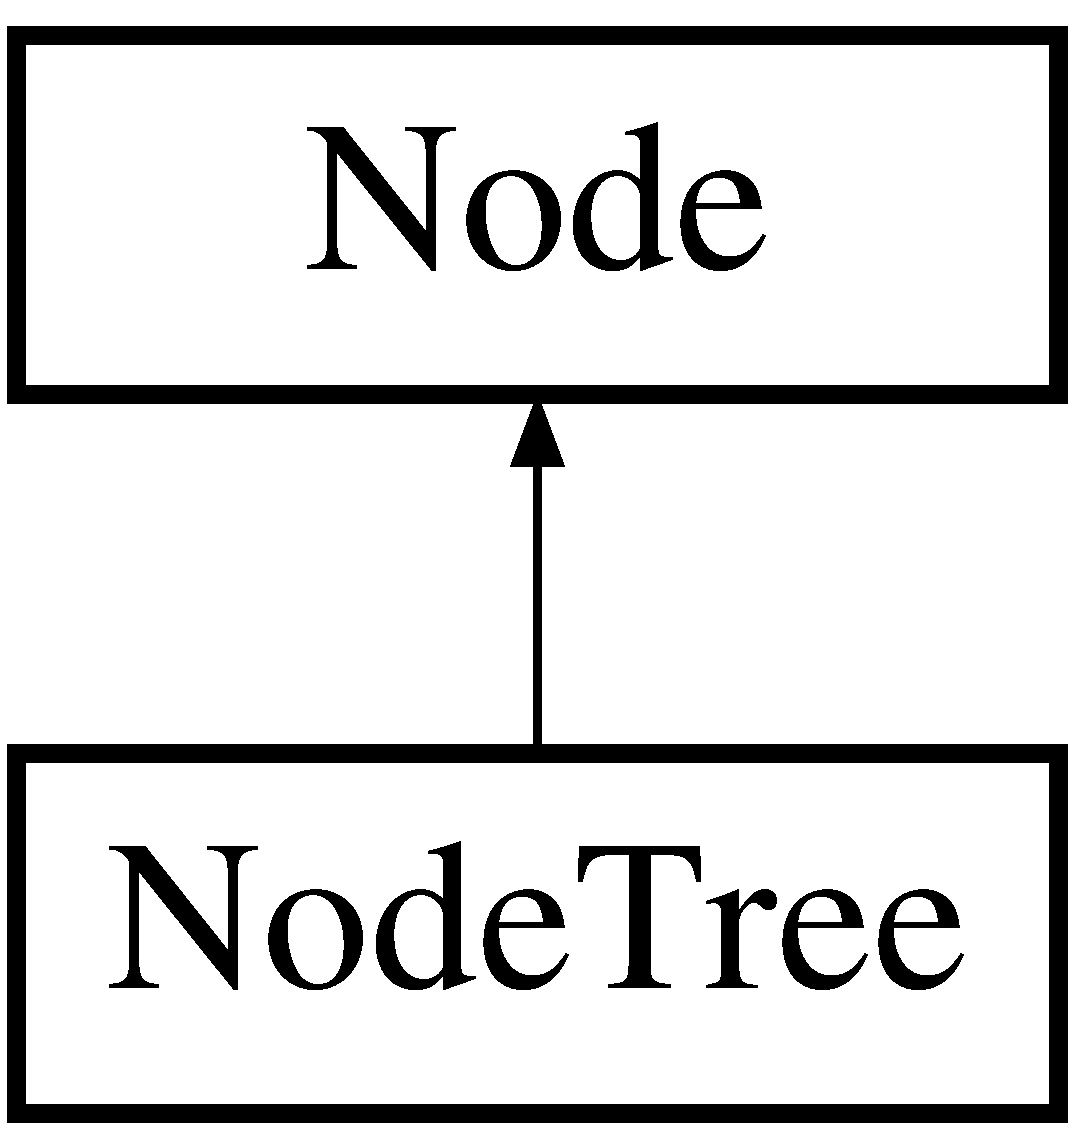
\includegraphics[height=2.000000cm]{class_node_tree}
\end{center}
\end{figure}
\subsection*{Public Member Functions}
\begin{DoxyCompactItemize}
\item 
\mbox{\Hypertarget{class_node_tree_aaffe7d72c1e5c56881854487370281a8}\label{class_node_tree_aaffe7d72c1e5c56881854487370281a8}} 
\mbox{\hyperlink{class_node_tree_aaffe7d72c1e5c56881854487370281a8}{Node\+Tree}} ()
\begin{DoxyCompactList}\small\item\em The Default constructor for the \mbox{\hyperlink{class_node_tree}{Node\+Tree}}. \end{DoxyCompactList}\item 
\mbox{\Hypertarget{class_node_tree_a6cb351a862dce80510ac48d145de2e9c}\label{class_node_tree_a6cb351a862dce80510ac48d145de2e9c}} 
{\bfseries Node\+Tree} (const int \&root\+Item)
\item 
\mbox{\Hypertarget{class_node_tree_a801678afd7b236bc75687a776e979f80}\label{class_node_tree_a801678afd7b236bc75687a776e979f80}} 
{\bfseries Node\+Tree} (const \mbox{\hyperlink{class_node_tree}{Node\+Tree}} \&tree)
\item 
\mbox{\hyperlink{class_node}{Node}} $\ast$ \mbox{\hyperlink{class_node_tree_ae6d1c0d70fc02fea199e9e7a81491d83}{insert\+Inorder}} (\mbox{\hyperlink{class_node}{Node}} $\ast$sub\+Tree\+Ptr, \mbox{\hyperlink{class_node}{Node}} $\ast$new\+Node)
\begin{DoxyCompactList}\small\item\em global variable to count the amount of nodes \end{DoxyCompactList}\item 
\mbox{\hyperlink{class_node}{Node}} $\ast$ \mbox{\hyperlink{class_node_tree_a5581b1e229d7310960e826a14e34f560}{get\+Root\+Ptr}} ()
\item 
virtual \mbox{\hyperlink{class_node_tree_a3ad091290982424bcc0750da7133e411}{$\sim$\+Node\+Tree}} ()
\item 
bool \mbox{\hyperlink{class_node_tree_a484735008677b458037b1ce114d12f1a}{is\+Empty}} (\mbox{\hyperlink{class_node}{Node}} $\ast$node\+Ptr) const
\begin{DoxyCompactList}\small\item\em Will test if the tree is empty. \end{DoxyCompactList}\item 
int \mbox{\hyperlink{class_node_tree_a711fa23ec5715b82c1a6dee780fde087}{get\+Height}} ()
\begin{DoxyCompactList}\small\item\em Will get the height by calling the helper. \end{DoxyCompactList}\item 
int \mbox{\hyperlink{class_node_tree_a504b5d012ccee99b85642d699396dd8f}{height\+Helper}} (\mbox{\hyperlink{class_node}{Node}} $\ast$tree\+Ptr)
\item 
int \mbox{\hyperlink{class_node_tree_ab619ff00f2cd2362d393ad41f2844129}{get\+Numberof\+Nodes}} (\mbox{\hyperlink{class_node}{Node}} $\ast$node\+Ptr) const
\begin{DoxyCompactList}\small\item\em Will return the number of nodes in the tree. It will run until both children get null. \end{DoxyCompactList}\item 
\mbox{\Hypertarget{class_node_tree_a037b369c78e107b423090eab320b022f}\label{class_node_tree_a037b369c78e107b423090eab320b022f}} 
int {\bfseries get\+Root\+Data} ()
\item 
\mbox{\Hypertarget{class_node_tree_aa1a0aebabeac588fe08b3fb810fe74ba}\label{class_node_tree_aa1a0aebabeac588fe08b3fb810fe74ba}} 
bool {\bfseries remove} (const int \&data)
\item 
void \mbox{\hyperlink{class_node_tree_aa354f6975e4e1123b47a21948d00e1b2}{set\+Root\+Data}} (const int \&new\+Data)
\item 
void \mbox{\hyperlink{class_node_tree_adfa34cb3970d7ea5ed4c7861ee844b1e}{set\+Root}} (\mbox{\hyperlink{class_node}{Node}} $\ast$root)
\item 
bool \mbox{\hyperlink{class_node_tree_a2e2cd480e0a50d94d26b09cfd721ac7a}{add}} (const int \&new\+Data)
\item 
void \mbox{\hyperlink{class_node_tree_a22be831083f6970a7ba6b64fcd0995ff}{clear}} (\mbox{\hyperlink{class_node}{Node}} $\ast$node\+Ptr)
\item 
int \mbox{\hyperlink{class_node_tree_a28bcd072ea53a04712a792b6b427371c}{get\+Entry}} (const int \&an\+Entry)
\begin{DoxyCompactList}\small\item\em Will find the entry and return the value, if not it will return 0. \end{DoxyCompactList}\item 
bool \mbox{\hyperlink{class_node_tree_a7a0617d6f4b39f495da71613a05a098e}{contains}} (const int \&an\+Entry) const
\item 
void \mbox{\hyperlink{class_node_tree_a73bd5a18b76a3741fcf49e0465622de2}{preorder\+Transverse}} (\mbox{\hyperlink{class_node}{Node}} $\ast$node\+Ptr) const
\begin{DoxyCompactList}\small\item\em Will preorder transverse the tree and print the data. \end{DoxyCompactList}\item 
void \mbox{\hyperlink{class_node_tree_a3973627c8a390da9b12e4bc9d4a9327d}{inorder\+Transverse}} (\mbox{\hyperlink{class_node}{Node}} $\ast$node\+Ptr) const
\begin{DoxyCompactList}\small\item\em Will inorder transverse the tree and print the data. \end{DoxyCompactList}\item 
void \mbox{\hyperlink{class_node_tree_a09ddf9e2cb245c50952b9669fb328907}{postorder\+Transverse}} (\mbox{\hyperlink{class_node}{Node}} $\ast$node\+Ptr) const
\begin{DoxyCompactList}\small\item\em Will postorder transverse the tree and print the data. \end{DoxyCompactList}\item 
\mbox{\hyperlink{class_node}{Node}} $\ast$ \mbox{\hyperlink{class_node_tree_a4a02f5a4836ed05e0d51e946101982b8}{delete\+Node}} (\mbox{\hyperlink{class_node}{Node}} $\ast$node\+Ptr, int key)
\begin{DoxyCompactList}\small\item\em Will delete the node with the key. \end{DoxyCompactList}\item 
\mbox{\hyperlink{class_node}{Node}} $\ast$ \mbox{\hyperlink{class_node_tree_a71a5469b3871672b409224ee905540c3}{min\+Value}} (\mbox{\hyperlink{class_node}{Node}} $\ast$node\+Ptr)
\item 
void \mbox{\hyperlink{class_node_tree_a4deaf904f4b727579020bcf6cba77a8f}{reset\+Count}} ()
\item 
void \mbox{\hyperlink{class_node_tree_ac57c84edf2b16c3fed7085413b272a62}{inorder\+Delete}} (\mbox{\hyperlink{class_node}{Node}} $\ast$node\+Ptr, int)
\begin{DoxyCompactList}\small\item\em Will delete the nodes that are equal to the nodes in B\+T\+S2. \end{DoxyCompactList}\end{DoxyCompactItemize}
\subsection*{Protected Member Functions}
\begin{DoxyCompactItemize}
\item 
\mbox{\hyperlink{class_node}{Node}} $\ast$ \mbox{\hyperlink{class_node_tree_a5f976e7369dcc91276df40678b59c33c}{remove\+Value}} (\mbox{\hyperlink{class_node}{Node}} $\ast$sub\+Tree\+Ptr, int target, bool \&success)
\item 
\mbox{\hyperlink{class_node}{Node}} $\ast$ \mbox{\hyperlink{class_node_tree_a68eae12d4ddd719e761e9e96211c8568}{remove\+Node}} (\mbox{\hyperlink{class_node}{Node}} $\ast$node\+Ptr)
\begin{DoxyCompactList}\small\item\em Will remove the node. \end{DoxyCompactList}\item 
\mbox{\hyperlink{class_node}{Node}} $\ast$ \mbox{\hyperlink{class_node_tree_a56b97fb5f2ea3ed32ec901e1a5589f89}{remove\+Leftmost\+Node}} (\mbox{\hyperlink{class_node}{Node}} $\ast$sub\+Tree\+Ptr, int \&inorder\+Successor)
\item 
\mbox{\hyperlink{class_node}{Node}} $\ast$ \mbox{\hyperlink{class_node_tree_a3f5897a41812b5694c57140eb5ade884}{find\+Node}} (\mbox{\hyperlink{class_node}{Node}} $\ast$tree\+Ptr, const int \&target) const
\begin{DoxyCompactList}\small\item\em Will find the node with that value and return the address of it. \end{DoxyCompactList}\end{DoxyCompactItemize}


\subsection{Constructor \& Destructor Documentation}
\mbox{\Hypertarget{class_node_tree_a3ad091290982424bcc0750da7133e411}\label{class_node_tree_a3ad091290982424bcc0750da7133e411}} 
\index{Node\+Tree@{Node\+Tree}!````~Node\+Tree@{$\sim$\+Node\+Tree}}
\index{````~Node\+Tree@{$\sim$\+Node\+Tree}!Node\+Tree@{Node\+Tree}}
\subsubsection{\texorpdfstring{$\sim$\+Node\+Tree()}{~NodeTree()}}
{\footnotesize\ttfamily Node\+Tree\+::$\sim$\+Node\+Tree (\begin{DoxyParamCaption}{ }\end{DoxyParamCaption})\hspace{0.3cm}{\ttfamily [virtual]}}

Destructor and will call clear to delete the nodes 

\subsection{Member Function Documentation}
\mbox{\Hypertarget{class_node_tree_a2e2cd480e0a50d94d26b09cfd721ac7a}\label{class_node_tree_a2e2cd480e0a50d94d26b09cfd721ac7a}} 
\index{Node\+Tree@{Node\+Tree}!add@{add}}
\index{add@{add}!Node\+Tree@{Node\+Tree}}
\subsubsection{\texorpdfstring{add()}{add()}}
{\footnotesize\ttfamily bool Node\+Tree\+::add (\begin{DoxyParamCaption}\item[{const int \&}]{new\+Data }\end{DoxyParamCaption})}

This is the function used to call the insert\+Inorder function 
\begin{DoxyParams}{Parameters}
{\em new\+Data} & \\
\hline
\end{DoxyParams}
\begin{DoxyReturn}{Returns}
true 
\end{DoxyReturn}
\begin{DoxyPrecond}{Precondition}
It will take the new data member to give to the insert 
\end{DoxyPrecond}
\begin{DoxyPostcond}{Postcondition}
Will create a new node with the data member in it. Then it will pass that new node and the root ptr to add to the tree 
\end{DoxyPostcond}
\mbox{\Hypertarget{class_node_tree_a22be831083f6970a7ba6b64fcd0995ff}\label{class_node_tree_a22be831083f6970a7ba6b64fcd0995ff}} 
\index{Node\+Tree@{Node\+Tree}!clear@{clear}}
\index{clear@{clear}!Node\+Tree@{Node\+Tree}}
\subsubsection{\texorpdfstring{clear()}{clear()}}
{\footnotesize\ttfamily void Node\+Tree\+::clear (\begin{DoxyParamCaption}\item[{\mbox{\hyperlink{class_node}{Node}} $\ast$}]{node\+Ptr }\end{DoxyParamCaption})}

Will recursively call itself to clear all the children and delete the root 
\begin{DoxyParams}{Parameters}
{\em node\+Ptr} & \\
\hline
\end{DoxyParams}
\begin{DoxyPrecond}{Precondition}
Will take in the root 
\end{DoxyPrecond}
\begin{DoxyPostcond}{Postcondition}
Will clear all the children and nodes recursively 
\end{DoxyPostcond}
\mbox{\Hypertarget{class_node_tree_a7a0617d6f4b39f495da71613a05a098e}\label{class_node_tree_a7a0617d6f4b39f495da71613a05a098e}} 
\index{Node\+Tree@{Node\+Tree}!contains@{contains}}
\index{contains@{contains}!Node\+Tree@{Node\+Tree}}
\subsubsection{\texorpdfstring{contains()}{contains()}}
{\footnotesize\ttfamily bool Node\+Tree\+::contains (\begin{DoxyParamCaption}\item[{const int \&}]{an\+Entry }\end{DoxyParamCaption}) const}

Will check if the tree contains that value 
\begin{DoxyParams}{Parameters}
{\em an\+Entry} & \\
\hline
\end{DoxyParams}
\begin{DoxyReturn}{Returns}
bool 
\end{DoxyReturn}
\begin{DoxyPrecond}{Precondition}
Will take in a int value to find 
\end{DoxyPrecond}
\begin{DoxyPostcond}{Postcondition}
Will call findnode and if that node contains the entry it will return true, else false 
\end{DoxyPostcond}
\mbox{\Hypertarget{class_node_tree_a4a02f5a4836ed05e0d51e946101982b8}\label{class_node_tree_a4a02f5a4836ed05e0d51e946101982b8}} 
\index{Node\+Tree@{Node\+Tree}!delete\+Node@{delete\+Node}}
\index{delete\+Node@{delete\+Node}!Node\+Tree@{Node\+Tree}}
\subsubsection{\texorpdfstring{delete\+Node()}{deleteNode()}}
{\footnotesize\ttfamily \mbox{\hyperlink{class_node}{Node}} $\ast$ Node\+Tree\+::delete\+Node (\begin{DoxyParamCaption}\item[{\mbox{\hyperlink{class_node}{Node}} $\ast$}]{node\+Ptr,  }\item[{int}]{key }\end{DoxyParamCaption})}



Will delete the node with the key. 


\begin{DoxyParams}{Parameters}
{\em node\+Ptr} & \\
\hline
{\em key} & \\
\hline
\end{DoxyParams}
\begin{DoxyReturn}{Returns}
node\+Ptr 
\end{DoxyReturn}
\begin{DoxyPrecond}{Precondition}
Will take in the root and key to delete that node 
\end{DoxyPrecond}
\begin{DoxyPostcond}{Postcondition}
Will recursively call itself and set the children to the correct places after the deletion 
\end{DoxyPostcond}
\mbox{\Hypertarget{class_node_tree_a3f5897a41812b5694c57140eb5ade884}\label{class_node_tree_a3f5897a41812b5694c57140eb5ade884}} 
\index{Node\+Tree@{Node\+Tree}!find\+Node@{find\+Node}}
\index{find\+Node@{find\+Node}!Node\+Tree@{Node\+Tree}}
\subsubsection{\texorpdfstring{find\+Node()}{findNode()}}
{\footnotesize\ttfamily \mbox{\hyperlink{class_node}{Node}} $\ast$ Node\+Tree\+::find\+Node (\begin{DoxyParamCaption}\item[{\mbox{\hyperlink{class_node}{Node}} $\ast$}]{tree\+Ptr,  }\item[{const int \&}]{target }\end{DoxyParamCaption}) const\hspace{0.3cm}{\ttfamily [protected]}}



Will find the node with that value and return the address of it. 


\begin{DoxyParams}{Parameters}
{\em tree\+Ptr} & \\
\hline
{\em target} & \\
\hline
\end{DoxyParams}
\begin{DoxyReturn}{Returns}
tree\+Ptr, will return the address to that target 
\end{DoxyReturn}
\begin{DoxyPrecond}{Precondition}
Will take in the root and the taret to find it 
\end{DoxyPrecond}
\begin{DoxyPostcond}{Postcondition}
Will recursively find the target and return the address of the node 
\end{DoxyPostcond}
\mbox{\Hypertarget{class_node_tree_a28bcd072ea53a04712a792b6b427371c}\label{class_node_tree_a28bcd072ea53a04712a792b6b427371c}} 
\index{Node\+Tree@{Node\+Tree}!get\+Entry@{get\+Entry}}
\index{get\+Entry@{get\+Entry}!Node\+Tree@{Node\+Tree}}
\subsubsection{\texorpdfstring{get\+Entry()}{getEntry()}}
{\footnotesize\ttfamily int Node\+Tree\+::get\+Entry (\begin{DoxyParamCaption}\item[{const int \&}]{an\+Entry }\end{DoxyParamCaption})}



Will find the entry and return the value, if not it will return 0. 


\begin{DoxyParams}{Parameters}
{\em an\+Entry} & \\
\hline
\end{DoxyParams}
\begin{DoxyReturn}{Returns}
an\+Entry 
\end{DoxyReturn}
\begin{DoxyPrecond}{Precondition}
Will take in a int value to pass to findnode 
\end{DoxyPrecond}
\begin{DoxyPostcond}{Postcondition}
Will call findnode to get the item, and if its the same it will return that value, if not it will return 0 
\end{DoxyPostcond}
\mbox{\Hypertarget{class_node_tree_a711fa23ec5715b82c1a6dee780fde087}\label{class_node_tree_a711fa23ec5715b82c1a6dee780fde087}} 
\index{Node\+Tree@{Node\+Tree}!get\+Height@{get\+Height}}
\index{get\+Height@{get\+Height}!Node\+Tree@{Node\+Tree}}
\subsubsection{\texorpdfstring{get\+Height()}{getHeight()}}
{\footnotesize\ttfamily int Node\+Tree\+::get\+Height (\begin{DoxyParamCaption}{ }\end{DoxyParamCaption})}



Will get the height by calling the helper. 

\begin{DoxyReturn}{Returns}
The int value given by the helper 
\end{DoxyReturn}
\begin{DoxyPrecond}{Precondition}

\end{DoxyPrecond}
\begin{DoxyPostcond}{Postcondition}
Will chall the helper function to return the number 
\end{DoxyPostcond}
\mbox{\Hypertarget{class_node_tree_ab619ff00f2cd2362d393ad41f2844129}\label{class_node_tree_ab619ff00f2cd2362d393ad41f2844129}} 
\index{Node\+Tree@{Node\+Tree}!get\+Numberof\+Nodes@{get\+Numberof\+Nodes}}
\index{get\+Numberof\+Nodes@{get\+Numberof\+Nodes}!Node\+Tree@{Node\+Tree}}
\subsubsection{\texorpdfstring{get\+Numberof\+Nodes()}{getNumberofNodes()}}
{\footnotesize\ttfamily int Node\+Tree\+::get\+Numberof\+Nodes (\begin{DoxyParamCaption}\item[{\mbox{\hyperlink{class_node}{Node}} $\ast$}]{node\+Ptr }\end{DoxyParamCaption}) const}



Will return the number of nodes in the tree. It will run until both children get null. 


\begin{DoxyParams}{Parameters}
{\em node\+Ptr} & \\
\hline
\end{DoxyParams}
\begin{DoxyReturn}{Returns}
nodes 
\end{DoxyReturn}
\begin{DoxyPrecond}{Precondition}
Will take the rootptr 
\end{DoxyPrecond}
\begin{DoxyPostcond}{Postcondition}
Will recursively call itself and increment the node counter to return the total value. 
\end{DoxyPostcond}
\mbox{\Hypertarget{class_node_tree_a5581b1e229d7310960e826a14e34f560}\label{class_node_tree_a5581b1e229d7310960e826a14e34f560}} 
\index{Node\+Tree@{Node\+Tree}!get\+Root\+Ptr@{get\+Root\+Ptr}}
\index{get\+Root\+Ptr@{get\+Root\+Ptr}!Node\+Tree@{Node\+Tree}}
\subsubsection{\texorpdfstring{get\+Root\+Ptr()}{getRootPtr()}}
{\footnotesize\ttfamily \mbox{\hyperlink{class_node}{Node}} $\ast$ Node\+Tree\+::get\+Root\+Ptr (\begin{DoxyParamCaption}{ }\end{DoxyParamCaption})}

Will return the root\+Ptr \begin{DoxyReturn}{Returns}
root\+Ptr 
\end{DoxyReturn}
\mbox{\Hypertarget{class_node_tree_a504b5d012ccee99b85642d699396dd8f}\label{class_node_tree_a504b5d012ccee99b85642d699396dd8f}} 
\index{Node\+Tree@{Node\+Tree}!height\+Helper@{height\+Helper}}
\index{height\+Helper@{height\+Helper}!Node\+Tree@{Node\+Tree}}
\subsubsection{\texorpdfstring{height\+Helper()}{heightHelper()}}
{\footnotesize\ttfamily int Node\+Tree\+::height\+Helper (\begin{DoxyParamCaption}\item[{\mbox{\hyperlink{class_node}{Node}} $\ast$}]{tree\+Ptr }\end{DoxyParamCaption})}

The height\+Helper because it can access the root\+Ptr itself 
\begin{DoxyParams}{Parameters}
{\em tree\+Ptr} & \\
\hline
\end{DoxyParams}
\begin{DoxyReturn}{Returns}
the max height 
\end{DoxyReturn}
\begin{DoxyPrecond}{Precondition}
Will take the rootptr to pass to the children 
\end{DoxyPrecond}
\begin{DoxyPostcond}{Postcondition}
Will recusievly call itself until if finds the nullptr, it will increment itself when it calls itself and returns the max number 
\end{DoxyPostcond}
\mbox{\Hypertarget{class_node_tree_ac57c84edf2b16c3fed7085413b272a62}\label{class_node_tree_ac57c84edf2b16c3fed7085413b272a62}} 
\index{Node\+Tree@{Node\+Tree}!inorder\+Delete@{inorder\+Delete}}
\index{inorder\+Delete@{inorder\+Delete}!Node\+Tree@{Node\+Tree}}
\subsubsection{\texorpdfstring{inorder\+Delete()}{inorderDelete()}}
{\footnotesize\ttfamily void Node\+Tree\+::inorder\+Delete (\begin{DoxyParamCaption}\item[{\mbox{\hyperlink{class_node}{Node}} $\ast$}]{node\+Ptr,  }\item[{int}]{key }\end{DoxyParamCaption})}



Will delete the nodes that are equal to the nodes in B\+T\+S2. 


\begin{DoxyParams}{Parameters}
{\em node\+Ptr} & \\
\hline
{\em key} & \\
\hline
\end{DoxyParams}
\begin{DoxyPrecond}{Precondition}
Will take the root and the key 
\end{DoxyPrecond}
\begin{DoxyPostcond}{Postcondition}
Will check if the key and the item in that node are equal, if equal it will call delete node to delete that node 
\end{DoxyPostcond}
\mbox{\Hypertarget{class_node_tree_a3973627c8a390da9b12e4bc9d4a9327d}\label{class_node_tree_a3973627c8a390da9b12e4bc9d4a9327d}} 
\index{Node\+Tree@{Node\+Tree}!inorder\+Transverse@{inorder\+Transverse}}
\index{inorder\+Transverse@{inorder\+Transverse}!Node\+Tree@{Node\+Tree}}
\subsubsection{\texorpdfstring{inorder\+Transverse()}{inorderTransverse()}}
{\footnotesize\ttfamily void Node\+Tree\+::inorder\+Transverse (\begin{DoxyParamCaption}\item[{\mbox{\hyperlink{class_node}{Node}} $\ast$}]{node\+Ptr }\end{DoxyParamCaption}) const}



Will inorder transverse the tree and print the data. 


\begin{DoxyParams}{Parameters}
{\em node\+Ptr} & \\
\hline
\end{DoxyParams}
\begin{DoxyPrecond}{Precondition}
Will get the rootptr to transverse the data 
\end{DoxyPrecond}
\begin{DoxyPostcond}{Postcondition}
Will recursively call itself to move through the tree to print it in inorder 
\end{DoxyPostcond}
\mbox{\Hypertarget{class_node_tree_ae6d1c0d70fc02fea199e9e7a81491d83}\label{class_node_tree_ae6d1c0d70fc02fea199e9e7a81491d83}} 
\index{Node\+Tree@{Node\+Tree}!insert\+Inorder@{insert\+Inorder}}
\index{insert\+Inorder@{insert\+Inorder}!Node\+Tree@{Node\+Tree}}
\subsubsection{\texorpdfstring{insert\+Inorder()}{insertInorder()}}
{\footnotesize\ttfamily \mbox{\hyperlink{class_node}{Node}} $\ast$ Node\+Tree\+::insert\+Inorder (\begin{DoxyParamCaption}\item[{\mbox{\hyperlink{class_node}{Node}} $\ast$}]{sub\+Tree\+Ptr,  }\item[{\mbox{\hyperlink{class_node}{Node}} $\ast$}]{new\+Node }\end{DoxyParamCaption})}



global variable to count the amount of nodes 

Will insert the values into the tree 
\begin{DoxyParams}{Parameters}
{\em sub\+Tree\+Ptr,pointer} & to the root \\
\hline
{\em new\+Node,pointer} & the a new\+Node that contains new value \\
\hline
\end{DoxyParams}
\begin{DoxyReturn}{Returns}
A pointer to the root 
\end{DoxyReturn}
\begin{DoxyPrecond}{Precondition}
Will take in the root pointer and a new node containing the value of the new value 
\end{DoxyPrecond}
\begin{DoxyPostcond}{Postcondition}
Will take the root pointer and the new node and set the new node to the right place 
\end{DoxyPostcond}
\mbox{\Hypertarget{class_node_tree_a484735008677b458037b1ce114d12f1a}\label{class_node_tree_a484735008677b458037b1ce114d12f1a}} 
\index{Node\+Tree@{Node\+Tree}!is\+Empty@{is\+Empty}}
\index{is\+Empty@{is\+Empty}!Node\+Tree@{Node\+Tree}}
\subsubsection{\texorpdfstring{is\+Empty()}{isEmpty()}}
{\footnotesize\ttfamily bool Node\+Tree\+::is\+Empty (\begin{DoxyParamCaption}\item[{\mbox{\hyperlink{class_node}{Node}} $\ast$}]{node\+Ptr }\end{DoxyParamCaption}) const}



Will test if the tree is empty. 


\begin{DoxyParams}{Parameters}
{\em node\+Ptr} & \\
\hline
\end{DoxyParams}
\begin{DoxyReturn}{Returns}
bool, if it is empty 
\end{DoxyReturn}
\begin{DoxyPrecond}{Precondition}
Will take in the root pointer 
\end{DoxyPrecond}
\begin{DoxyPostcond}{Postcondition}
Will recursively check if the node points to null, or both children are null 
\end{DoxyPostcond}
\mbox{\Hypertarget{class_node_tree_a71a5469b3871672b409224ee905540c3}\label{class_node_tree_a71a5469b3871672b409224ee905540c3}} 
\index{Node\+Tree@{Node\+Tree}!min\+Value@{min\+Value}}
\index{min\+Value@{min\+Value}!Node\+Tree@{Node\+Tree}}
\subsubsection{\texorpdfstring{min\+Value()}{minValue()}}
{\footnotesize\ttfamily \mbox{\hyperlink{class_node}{Node}} $\ast$ Node\+Tree\+::min\+Value (\begin{DoxyParamCaption}\item[{\mbox{\hyperlink{class_node}{Node}} $\ast$}]{node\+Ptr }\end{DoxyParamCaption})}

Will find the min value in the tree 
\begin{DoxyParams}{Parameters}
{\em node\+Ptr} & \\
\hline
\end{DoxyParams}
\begin{DoxyReturn}{Returns}
current, pointer to the address of the min value 
\end{DoxyReturn}
\begin{DoxyPrecond}{Precondition}
Will take in the root to find the mon value 
\end{DoxyPrecond}
\begin{DoxyPostcond}{Postcondition}
Will run down the left pointers until it finds null and return the address where it is min value 
\end{DoxyPostcond}
\mbox{\Hypertarget{class_node_tree_a09ddf9e2cb245c50952b9669fb328907}\label{class_node_tree_a09ddf9e2cb245c50952b9669fb328907}} 
\index{Node\+Tree@{Node\+Tree}!postorder\+Transverse@{postorder\+Transverse}}
\index{postorder\+Transverse@{postorder\+Transverse}!Node\+Tree@{Node\+Tree}}
\subsubsection{\texorpdfstring{postorder\+Transverse()}{postorderTransverse()}}
{\footnotesize\ttfamily void Node\+Tree\+::postorder\+Transverse (\begin{DoxyParamCaption}\item[{\mbox{\hyperlink{class_node}{Node}} $\ast$}]{node\+Ptr }\end{DoxyParamCaption}) const}



Will postorder transverse the tree and print the data. 


\begin{DoxyParams}{Parameters}
{\em node\+Ptr} & \\
\hline
\end{DoxyParams}
\begin{DoxyPrecond}{Precondition}
Will get the rootptr to transverse the data 
\end{DoxyPrecond}
\begin{DoxyPostcond}{Postcondition}
Will recursively call itself to move through the tree to print it in postorder 
\end{DoxyPostcond}
\mbox{\Hypertarget{class_node_tree_a73bd5a18b76a3741fcf49e0465622de2}\label{class_node_tree_a73bd5a18b76a3741fcf49e0465622de2}} 
\index{Node\+Tree@{Node\+Tree}!preorder\+Transverse@{preorder\+Transverse}}
\index{preorder\+Transverse@{preorder\+Transverse}!Node\+Tree@{Node\+Tree}}
\subsubsection{\texorpdfstring{preorder\+Transverse()}{preorderTransverse()}}
{\footnotesize\ttfamily void Node\+Tree\+::preorder\+Transverse (\begin{DoxyParamCaption}\item[{\mbox{\hyperlink{class_node}{Node}} $\ast$}]{node\+Ptr }\end{DoxyParamCaption}) const}



Will preorder transverse the tree and print the data. 


\begin{DoxyParams}{Parameters}
{\em node\+Ptr} & \\
\hline
\end{DoxyParams}
\begin{DoxyPrecond}{Precondition}
Will get the rootptr to transverse the data 
\end{DoxyPrecond}
\begin{DoxyPostcond}{Postcondition}
Will recursively call itself to move through the tree to print it in preorder 
\end{DoxyPostcond}
\mbox{\Hypertarget{class_node_tree_a56b97fb5f2ea3ed32ec901e1a5589f89}\label{class_node_tree_a56b97fb5f2ea3ed32ec901e1a5589f89}} 
\index{Node\+Tree@{Node\+Tree}!remove\+Leftmost\+Node@{remove\+Leftmost\+Node}}
\index{remove\+Leftmost\+Node@{remove\+Leftmost\+Node}!Node\+Tree@{Node\+Tree}}
\subsubsection{\texorpdfstring{remove\+Leftmost\+Node()}{removeLeftmostNode()}}
{\footnotesize\ttfamily \mbox{\hyperlink{class_node}{Node}} $\ast$ Node\+Tree\+::remove\+Leftmost\+Node (\begin{DoxyParamCaption}\item[{\mbox{\hyperlink{class_node}{Node}} $\ast$}]{sub\+Tree\+Ptr,  }\item[{int \&}]{inorder\+Successor }\end{DoxyParamCaption})\hspace{0.3cm}{\ttfamily [protected]}}

Will remove the left most \mbox{\hyperlink{class_node}{Node}} 
\begin{DoxyParams}{Parameters}
{\em sub\+Tree\+Ptr} & \\
\hline
{\em inorder\+Successor} & \\
\hline
\end{DoxyParams}
\begin{DoxyReturn}{Returns}
will wall the remove node to remove that node 
\end{DoxyReturn}
\begin{DoxyPrecond}{Precondition}
Will take in the root pointer and the value to set it 
\end{DoxyPrecond}
\begin{DoxyPostcond}{Postcondition}
Will get traverse to get to the left most node and then call remove\+Node to delete it 
\end{DoxyPostcond}
\mbox{\Hypertarget{class_node_tree_a68eae12d4ddd719e761e9e96211c8568}\label{class_node_tree_a68eae12d4ddd719e761e9e96211c8568}} 
\index{Node\+Tree@{Node\+Tree}!remove\+Node@{remove\+Node}}
\index{remove\+Node@{remove\+Node}!Node\+Tree@{Node\+Tree}}
\subsubsection{\texorpdfstring{remove\+Node()}{removeNode()}}
{\footnotesize\ttfamily \mbox{\hyperlink{class_node}{Node}} $\ast$ Node\+Tree\+::remove\+Node (\begin{DoxyParamCaption}\item[{\mbox{\hyperlink{class_node}{Node}} $\ast$}]{node\+Ptr }\end{DoxyParamCaption})\hspace{0.3cm}{\ttfamily [protected]}}



Will remove the node. 


\begin{DoxyParams}{Parameters}
{\em node\+Ptr} & \\
\hline
\end{DoxyParams}
\begin{DoxyReturn}{Returns}
node\+Ptr 
\end{DoxyReturn}
\begin{DoxyPrecond}{Precondition}
Will take in the pointer to delete the node 
\end{DoxyPrecond}
\begin{DoxyPostcond}{Postcondition}
Will take the pointer and delete that node and then fill in the gap 
\end{DoxyPostcond}
\mbox{\Hypertarget{class_node_tree_a5f976e7369dcc91276df40678b59c33c}\label{class_node_tree_a5f976e7369dcc91276df40678b59c33c}} 
\index{Node\+Tree@{Node\+Tree}!remove\+Value@{remove\+Value}}
\index{remove\+Value@{remove\+Value}!Node\+Tree@{Node\+Tree}}
\subsubsection{\texorpdfstring{remove\+Value()}{removeValue()}}
{\footnotesize\ttfamily \mbox{\hyperlink{class_node}{Node}} $\ast$ Node\+Tree\+::remove\+Value (\begin{DoxyParamCaption}\item[{\mbox{\hyperlink{class_node}{Node}} $\ast$}]{sub\+Tree\+Ptr,  }\item[{int}]{target,  }\item[{bool \&}]{success }\end{DoxyParamCaption})\hspace{0.3cm}{\ttfamily [protected]}}

Will remove a value from the tree 
\begin{DoxyParams}{Parameters}
{\em sub\+Tree\+Ptr} & \\
\hline
{\em target} & \\
\hline
{\em success} & \\
\hline
\end{DoxyParams}
\begin{DoxyReturn}{Returns}
a pointer the the node 
\end{DoxyReturn}
\begin{DoxyPrecond}{Precondition}
Will take in the root , the target and the bool value 
\end{DoxyPrecond}
\begin{DoxyPostcond}{Postcondition}
It will recursively call itself to remove the target and return that pointer 
\end{DoxyPostcond}
\mbox{\Hypertarget{class_node_tree_a4deaf904f4b727579020bcf6cba77a8f}\label{class_node_tree_a4deaf904f4b727579020bcf6cba77a8f}} 
\index{Node\+Tree@{Node\+Tree}!reset\+Count@{reset\+Count}}
\index{reset\+Count@{reset\+Count}!Node\+Tree@{Node\+Tree}}
\subsubsection{\texorpdfstring{reset\+Count()}{resetCount()}}
{\footnotesize\ttfamily void Node\+Tree\+::reset\+Count (\begin{DoxyParamCaption}{ }\end{DoxyParamCaption})}

Will reset the node value for get\+Numberof\+Nodes \begin{DoxyPostcond}{Postcondition}
Will reset the global variable nodes to 1 
\end{DoxyPostcond}
\mbox{\Hypertarget{class_node_tree_adfa34cb3970d7ea5ed4c7861ee844b1e}\label{class_node_tree_adfa34cb3970d7ea5ed4c7861ee844b1e}} 
\index{Node\+Tree@{Node\+Tree}!set\+Root@{set\+Root}}
\index{set\+Root@{set\+Root}!Node\+Tree@{Node\+Tree}}
\subsubsection{\texorpdfstring{set\+Root()}{setRoot()}}
{\footnotesize\ttfamily void Node\+Tree\+::set\+Root (\begin{DoxyParamCaption}\item[{\mbox{\hyperlink{class_node}{Node}} $\ast$}]{root }\end{DoxyParamCaption})}

Will rest the root\+Ptr to a address 
\begin{DoxyParams}{Parameters}
{\em root} & \\
\hline
\end{DoxyParams}
\begin{DoxyPrecond}{Precondition}
Will take in a node pointer 
\end{DoxyPrecond}
\begin{DoxyPostcond}{Postcondition}
Will set the root\+Ptr to the root address 
\end{DoxyPostcond}
\mbox{\Hypertarget{class_node_tree_aa354f6975e4e1123b47a21948d00e1b2}\label{class_node_tree_aa354f6975e4e1123b47a21948d00e1b2}} 
\index{Node\+Tree@{Node\+Tree}!set\+Root\+Data@{set\+Root\+Data}}
\index{set\+Root\+Data@{set\+Root\+Data}!Node\+Tree@{Node\+Tree}}
\subsubsection{\texorpdfstring{set\+Root\+Data()}{setRootData()}}
{\footnotesize\ttfamily void Node\+Tree\+::set\+Root\+Data (\begin{DoxyParamCaption}\item[{const int \&}]{new\+Data }\end{DoxyParamCaption})}

Will set the s 
\begin{DoxyParams}{Parameters}
{\em new\+Data} & \\
\hline
\end{DoxyParams}
\begin{DoxyPrecond}{Precondition}
Will take in a in to give to the root ptr 
\end{DoxyPrecond}
\begin{DoxyPostcond}{Postcondition}
Will call the constructor for a new node and give the root pointer that data 
\end{DoxyPostcond}


The documentation for this class was generated from the following files\+:\begin{DoxyCompactItemize}
\item 
Node\+Tree.\+h\item 
Node\+Tree.\+cpp\end{DoxyCompactItemize}

%--- End generated contents ---

% Index
\backmatter
\newpage
\phantomsection
\clearemptydoublepage
\addcontentsline{toc}{chapter}{Index}
\printindex

\end{document}
